\documentclass[11pt,a4paper,oneside]{article}
\usepackage{titling}
\newcommand{\subtitle}[1]{%
  \posttitle{%
    \par\end{center}
    \begin{center}\large#1\end{center}
    \vskip0.5em}%
}
\title{\textbf{Group 21: Cognitive Modeling - Lab 3}}
\date{\today}
\author{Olusanmi Hundogan - 6883273\\
Evangelia Giannikou - 6988229\\
}
% \pagenumbering{gobble}
\pagenumbering{arabic}

% \usepackage{eurosym}
\usepackage{hyperref}
% \usepackage{subfig}
\usepackage{amsmath}
\usepackage{amssymb}
\usepackage{tabularx,booktabs}
\usepackage{multicol}
\usepackage{array}
\usepackage{float}
\usepackage[english]{babel}
\usepackage{wrapfig}
\usepackage{graphicx}
\usepackage[font=scriptsize]{caption}
\usepackage{subcaption}


\setcounter{secnumdepth}{0}
\newcolumntype{M}[1]{>{\centering\arraybackslash}m{#1}}
\usepackage[backend=biber, sorting=none]{biblatex}
\usepackage[margin=1in]{geometry}
\addbibresource{references.bib}

\newcommand{\icol}[1]{% inline column vector
  \left(\begin{smallmatrix}#1\end{smallmatrix}\right)%
}

\newcommand{\irow}[1]{% inline row vector
  \begin{smallmatrix}(#1)\end{smallmatrix}%
}

\begin{document}

\maketitle

\section{Question 1}
\label{Q1}
\subsection{Height: mean = 180, st.d = 10}
\textit{Show two graphs: (i) what the \textbf{probability} of using threshold looks like on the scale 1-250 cm; (ii) the graph of the function $\sigma$ on the same scale. State which degree point has the highest probability of being used as a threshold, and on which degree point it is most likely the speaker will use the adjective tall. If the two values differ or are the same, say in a few words why you think this is so.}\\

In Figure \ref{fig:q1_threshold}, the \textbf{probability} of using threshold on the scale 1-250 cm is shown. The highest degree point is when $ P(\Theta; \lambda; c) = 0.083$, and $\theta = 184$ cm.

\begin{figure}[H]
    \centering
    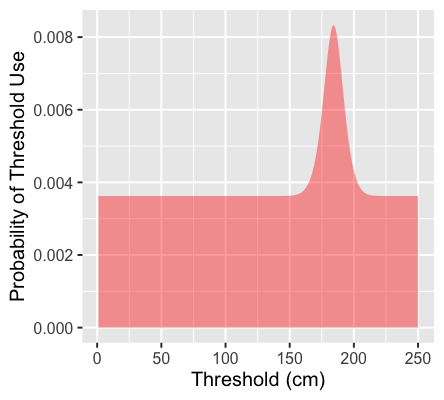
\includegraphics[width=100mm]{figs/Question_1_threshold.png}
    \caption{The graph shows the probability of threshold use on a scale of 1-250 cm.}
  \label{fig:q1_threshold}
\end{figure}

Similarly, in Figure \ref{fig:q1_sigma}, it is shown the graph of the function $\sigma$ on the same x-scale. The highest degree point is 1 and height = 250 cm. 250 yields the highest likelihood of adjective use. At this threshold, it is certain that if the speaker utters "tall" he will be referring to 250 and the listener will understand it as such. As the value decreases, the likelihood is diminishing as well.

\begin{figure}[H]
    \centering
    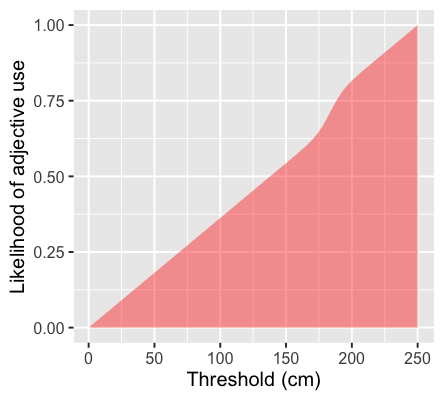
\includegraphics[width=100mm]{figs/Question_1_sigma.png}
    \caption{The graph shows the function $\sigma$ on a scale 1-250 cm.}
  \label{fig:q1_sigma}
\end{figure}

Comparing the two degree points to evaluate the communication efficiency, it is evident that the two values deviate. Considering that $\theta = 250$ is not efficient because it does not apply to a large population of people, the speaker is most likely to use 184 cm as threshold. For other values of $\theta$, someone described as "tall" would probably make it inefficient to use.

\section{Question 2}
\label{Q2}
\subsection{IQ - normal distribution}
\textit{Specify the normal distribution and generate figures for $ES$ and $\sigma$ function using this distribution and report which degree has the highest $ES$.}\\

For specifying the IQ distribution, we use $IQ \sim \mathcal{N}(100, 15)$ since $mean = 100$, given from the description, and with 95\% confidence interval $st.d. = 15$. 

\begin{figure}[H]
    \centering
    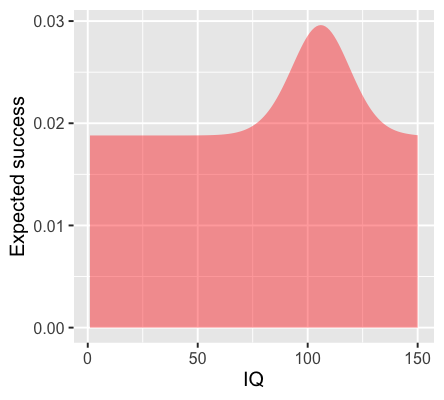
\includegraphics[width=100mm]{figs/Question_2_IQ_es.png}
    \caption{The graph shows the Expected Success function for IQ on a scale of 1-150.}
  \label{fig:q2_iq_es}
\end{figure}

The highest expected success $ES = 0.029$ in Figure \ref{fig:q2_iq_es} is at $IQ = 106$.


\begin{figure}[H]
    \centering
    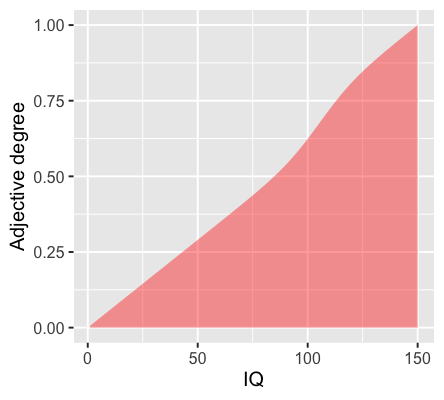
\includegraphics[width=100mm]{figs/Question_2_IQ_sigma.png}
    \caption{The graph shows the $\sigma$ function for IQ on a scale of 1-150.}
  \label{fig:q2_iq_sigma}
\end{figure}

The highest likelihood of adjective use $\sigma(A|d; \lambda; c) = 1$ in Figure \ref{fig:q2_iq_sigma} is at $IQ = 150$.


\subsection{Waiting times - gamma distribution}
\textit{Specify the gamma distribution and generate figures for $ES$ and $\sigma$. Report which degree has the highest $ES$.}\\

For specifying the waiting times distribution, we use Waiting times $\sim \mathcal{\gamma}(2, 1)$. These values were estimated by using $\frac{\mu^2}{\sigma^2}$ and $\frac{\sigma^2}{\mu}$ for the shape and scale parameters, respectively. 
%[TO-DO: explain more why these values]

\begin{figure}[H]
    \centering
    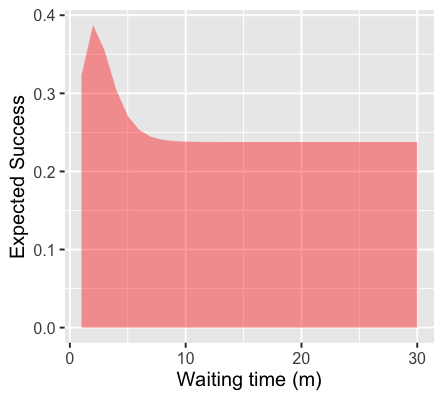
\includegraphics[width=100mm]{figs/Question_2_waiting_time_es.png}
    \caption{The graph shows the Expected Success function for waiting on a scale of 1-30.}
  \label{fig:q2_waiting_es}
\end{figure}

The highest expected success $ES = 0.387$ in Figure \ref{fig:q2_waiting_es} is at waiting time $= 2$ minutes.


\begin{figure}[H]
    \centering
    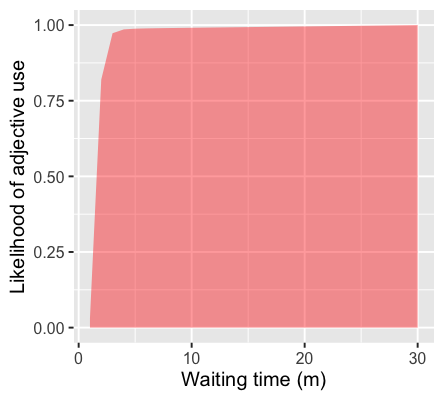
\includegraphics[width=100mm]{figs/Question_2_waiting_time_sigma.png}
    \caption{The graph shows the $\sigma$ function for waiting on a scale of 1-30.}
  \label{fig:q2_waiting_sigma}
\end{figure}
The highest likelihood of adjective use $\sigma(A|d; \lambda; c) = 1$ in Figure \ref{fig:q2_waiting_sigma} is at waiting time $= 30$ minutes.


\section{Question 3}
\label{Question 3}
\textit{What is Pearson’s correlation coefficient, r, between model’s predictions and actual observations. Check the value of $r$ with respect to three different parameters of the model (9 comparisons in total):}

\begin{itemize}
    \item \textit{lambda=40, coverage.parameter=0.1}
    \item \textit{lambda=40, coverage.parameter=-0.1}
    \item \textit{lambda=40, coverage.parameter=0}
\end{itemize}

\textit{What coverage parameter gives us the best and the worst linear correlation? On which distribution do we get the best results?}

\textit{Afterward, pick the coverage parameter that worked best and select two distributions by flipping their prior belief distributions. Report what prior distribution you used and report r. Do we see that r is affected? Does the model suffer in having worse linear correlation with respect to the observed data? Say in a few words why this is the case.}\\

As it is visible in Table \ref{question_3}, the best linear correlation is given when the coverage parameter is -0.1 in which the r value is on average $r = 0.97$. The worst correlation is given when coverage parameter is 0.1 in which the average correlation values is $r = 0.86$.

Similarly, when comparing the results between the distribution, the best correlation is that of the Left-skewed with an average of $r = 0.94$. The worst correlation is given for the Moved distribution in which the on average correlation is $r = 0.91$.

\begin{table}[ht]
\centering
\begin{tabular}{rccc}
  \hline
 Model & r when $c = 0.1$ & r when $c = -0.1$ & r when $c = 0$ \\ 
  \hline
    Gaussian & 0.88 & 0.97 & 0.94\\ 
    Left - skewed & 0.85 & 0.98 & 0.98\\ 
    Moved & 0.84 & 0.97 & 0.93\\ 
   \hline
\end{tabular}
\caption{Pearson's correlation between model's prediction and actual observation for 3 different model distributions where $\lambda = 40$ and coverage parameter is 0.1, -0.1 and 0.}
\label{question_3}
\end{table}

For the second part of the question, we picked $c = -0.1$ as the best coverage parameter and selected to flip the distribution of the left-skewed and moved models. In particular, we used $\mathcal{N}(6, 2)$ for the left-skewed model. The correlation we found was $r = 0.95$. For the moved model we used $\mathcal{\gamma}(4, 1.5)$. The correlation found was $r = 0.86$.

A sum of the results in regards to the previously observed data is found on  \autoref{question_3_flipped}. In the case of the left-skewed model, the correlation worsens slightly with a Gaussian prior distribution set. This decrease was expected since Gaussian distribution would not work well with data that are concentrated on the right side of the distribution. Given that the data distribution was generated under a different distribution, it makes sense that a differing prior distribution will be biased towards that prior distribution. Hence, the model will have difficulties adjusting to the data, while keeping the prior in mind. Similar holds for the moved distribution as it's underlying prior is Gaussian and a Gamma distribution would not fit well.


\begin{table}[ht]
\centering
\begin{tabular}{rccr}
  \hline
 Model & r with Normal distribution & r with Gamma distribution\\ 
  \hline
    Left - skewed & 0.95* & 0.98 \\ 
    Moved & 0.97 & 0.86* \\ 
   \hline
\end{tabular}
\caption{Pearson's correlation between 2 models with $c = -0.1$. R values with * indicate the new correlation values with flipped distribution.}
\label{question_3_flipped}
\end{table}

\section{Question 4} 
\label{Question 4}
\textit{Bayesian model - What values have been found for lambda and coverage.parameter? Report summary statistics on lambda and coverage.parameter (MAP, median, 2.5\% to 97.5\%). Discuss briefly the summaries.}\\

For the Bayesian model, we used as a prior $\mathcal{N}(6, 2)$. As seen in \autoref{question_4},  the values of 2.5\% and 97.5\% interval indicate the limits of c and $\lambda$. Hence, there is a 95\% chance that $ c \in [-0.332, -0.107]$ and $\lambda \in [18.483, 48.985]$. The MAP values are $c = -0.197$ and $\lambda = 33.364$. These values are very close to the ones we found in \autref{Question 3} ($\lambda = 40$, $c = -0.1$) for the highest correlation value given a Gaussian distribution. These estimates are reasonable in the context of the experiment as a negative coverage parameter hints that the gradable adjective is not generally applicable \cite{qing_MeaningUseGradable_2014}. Intuitively, this holds for an adjective like 'big'.


\begin{table}[ht]
\centering
\begin{tabular}{ccccc}
  \hline
  & MAP & median & 2.5\% interval & 97.5\% interval\\ 
  \hline
    c & -0.197 & -0.204 & -0.332 & -0.107\\ 
    $\lambda$ & 33.364 & 34.919 & 18.483 & 48.985\\ 
   \hline
\end{tabular}
\caption{A statistics summary of c and $\lambda$ for adjective='big' on a Gaussian distribution.}
\label{question_4}
\end{table}


\section{Question 5}
\label{Q5}
\textit{Expand your model to construct the posterior distribution of the two parameters using three adjectives (big, pointy, tall) in all three distributions. Explore the distribution of the parameters in \emph{out}. Plot the summary and report summary statistics on lambda and coverage.parameter.}\\

Similar to \autref{Question 4}, we used as a prior $\mathcal{N}(6, 2)$ for all three adjectives 'big','pointy' and 'tall'. Again, there is a 95\% chance that $ c \in [-0.045, -0.016]$ and $\lambda \in [25.764, 39.160]$. The MAP values are $c = -0.031$ and $\lambda = 30.788$ which are further away from $c = -0.01$ and $\lambda = 40$. The increased deviation is reasonable as we now expand the model to include three adjectives. Beforehand, the model only focused on the adjective "big". 

\begin{table}[ht]
\centering
\begin{tabular}{ccccc}
  \hline
  & MAP & median & 2.5\% interval & 97.5\% interval\\ 
  \hline
    c & -0.031 & -0.031 & -0.045  & -0.016\\ 
    $\lambda$ & 30.788 & 31.269 & 25.764  & 39.160\\ 
   \hline
\end{tabular}
\caption{A statistics summary of c and $\lambda$ for adjectives = 'big', 'pointy', 'tall' for 3 distributions.}
\label{question_5}
\end{table}

\section{Bonus question}
\label{bonus}
\textit{We specified the likelihood using dnorm with $sd=0.1$. Is this sensible or not? Check what dnorm is and state what problems there might be with this particular function and with $sd=0.1$ for our data. Is there an alternative probability distribution that would make more sense?}\\

The dnorm function returns a probability/density for a given value, a mean and a st.d. In our case the mean is determined by a data point in the experimental data set. Hence, the simulation collects the sum of each degrees percentage value for an adjective given their likelihood under their respective likelihood of adjective use.

The standard deviation determines how much samples "disperse" from the mean. A low value of st.d. as here, indicate that the data points tend to be close to the mean. A low value like 0.1 seems reasonable as the likelihoods of adjective use will remain within the bounds of the 0 and 1. Increasing the standard deviation increases the range of "highly" probable deviations. Reducing the st.d might not capture the unexplained variations within the data, that are necessary for a "faithful" simulation. Determining the correct standard distribution is therefore difficult.  

%However, 99\% of a normal distribution lie within 3 standard deviations from the mean. Meaning, that the data generated will only remain within valid bounds (0 to 1) if the means are within the range of .3 and .7. However, for means that exceed this range the simulation may often produce invalid values which are detrimental for the simulation. Choosing a smaller st.d may mitigate this issue slightly but it is not possible to overcome it. Furthermore, choosing the st.d to be too small, risks overfitting the basis data by producing simulated values that are to close to the initial data. 

As a result, choosing the normal distribution may not be the best approach to model the simulation. With most of the true data being left-skewed it makes more sense to model the generated data as random samples from a left-skewed distribution. This is further supported by the results from \autref{Question 3} which showed that the left-skewed gamma-prior produced results which correlated the most with the true data.
Moreover, in a left-skewed distribution, small data values are gathered on the left, whereas higher values are gathered to the right. This pattern also emerges from the likelihood of the adjective use. We can model the simulation in a similar way by 

% By keeping the data points concentrated to the mean, we ensure that the likehood's values will not be widespread. 

%the accuracy of someone using an adjective ?!



Second, because we want to ensure the communication efficiency.  Communication efficiency increases as the values of likelihood increase. Since we want a concentration of values on the ride side to increase communication efficiency, a left skewed distribution might be a better choice.

\clearpage 
\printbibliography
\end{document}